\documentclass[
  12pt,
  headsepline,
  headings=normal,
  toc=bibliography,
  toc=listof
]{scrreport}


%% Variabeln %%%%%%%%%%%%%%%%%%%%%%%%%%%%%%%%%%%%%%%%%%%%%%%%%%%%

\renewcommand{\author}{Guillaume Fournier-Mayer}
\renewcommand{\title}{Rechnergestützter Entwurf digitaler Systeme}

%\RedeclareSectionCommand[tocnumwidth=2.3em]{chapter}
%\RedeclareSectionCommand[tocindent=2.3em,tocnumwidth=3.2em]{section}
\setcounter{secnumdepth}{\subsubsectionnumdepth}
\setcounter{tocdepth}{3}


%% Documentclass Anpassungen
\usepackage{scrhack}


%% Deutsche Anpassungen %%%%%%%%%%%%%%%%%%%%%%%%%%%%%%%%%%%%%
\usepackage[ngerman]{babel}
\usepackage[EU1]{fontenc}
\usepackage[utf8]{inputenc}
\usepackage{lmodern} %Type1-Schriftart für nicht-englische Texte
\usepackage{textcomp}


%% Packages für Grafiken & Abbildungen %%%%%%%%%%%%%%%%%%%%%%
\usepackage{graphicx}
%\usepackage{eso-pic}
\usepackage{float}


%% Hyperref %%%%%%%%%%%%%%%%%%%%%%%%%%%%%%%%%%%%%%%%%%%%%%%%%
\usepackage[final, backref=false, pagebackref=false, bookmarks=true]{hyperref}

\hypersetup{ %Ä=\304; Ö=\326; Ü=\334; ä=\344; ö=\366; ü=\374; ß=\377
  pdfauthor={Guillaume Fournier-Mayer},
  pdftitle={EDA-Praktikum},
  pdfsubject={\title},
  pdfproducer={MiKTeX},
  pdfview=FitV,             % Fit, FitH, FitV
  pdfstartview=FitV,        % PDF-Viewer benutzt beim Start bestimmte Seitenbreite
                            % (Fit, FitH, FitV)
  pdfpagemode=UseOutlines,  % PDF-Viewer startet ohne Inhaltsverzeichnis et.al.
                            % (FullScreen, UseOutlines, None)
  linkcolor=black,          % Für Links in der gleichen Seite
  urlcolor=blue,            % Für Links auf URL’s
  breaklinks=false,         % Links dürfen umgebrochen werden
  colorlinks=true,
  citecolor=black,          % Farbe für \cite
  citebordercolor=0 0 0,
  filebordercolor=0 0 0,
  linkbordercolor=0 0 0,
  menubordercolor=0 0 0,
  urlbordercolor=0 0 0,
  pdfhighlight=/I,
  pdfborder=0 0 0,          % keine Box um die Links!
  bookmarksnumbered=false,
  hypertexnames=false,
  bookmarksopen=true
}

%% Geometry %%%%%%%%%%%%%%%%%%%%%%%%%%%%%%%%%%%%%%%%%%%%%%%%%
%\geometry{includeheadfoot, headheight = 17mm, textwidth = 16cm, textheight = 23cm}
\usepackage[left=35mm, right=30mm, top=30mm, bottom=30mm, a4paper]{geometry}

%% TABLE %%%%%%%%%%%%%%%%%%%%%%%%%%%%%%%%%%%%%%%%%%%%%%%%%%%
\usepackage{longtable}
\usepackage{multirow}
%% Header %%%%%%%%%%%%%%%%%%%%%%%%%%%%%%%%%%%%%%%%%%%%%%%%%%%
\usepackage[automark]{scrlayer-scrpage}
\pagestyle{scrheadings}
%\clearpairofpagestyles
\chead{}
\ihead{\headmark}
\automark{chapter}


%% Zitate %%%%%%%%%%%%%%%%%%%%%%%%%%%%%%%%%%%%%%%%%%%%%%%%%%%%%
\usepackage[backend=biber,style=numeric,]{biblatex}
\usepackage{csquotes}
\addbibresource{literatur.bib}
\usepackage{dirtytalk}

%% Formeln %%%%%%%%%%%%%%%%%%%%%%%%%%%%%%%%%%%%%%%%%%%%%%%%%%%%%
\usepackage{amsmath}
\usepackage{nicefrac}

%% Titel %%%%%%%%%%%%%%%%%%%%%%%%%%%%%%%%%%%%%%%%%%%%%%%%%%%%%

%% Dokument %%%%%%%%%%%%%%%%%%%%%%%%%%%%%%%%%%%%%%%%%%%%%%%%%%%%
\begin{document}
%\AddToShipoutPicture{\includegraphics{img/Deckblatt.pdf}}
\begin{titlepage}
  \begin{center}
    
\includegraphics[scale=0.15]{img/wedel_logo.png}\\
    \vspace{1cm}
    \begin{Huge}
      \textbf{\title}\\
    \end{Huge}
    \vspace{1cm}
    \begin{LARGE}
      Kräfteplazierung\\
    \end{LARGE}
    \begin{Large}
      Fachrichtung technische Informatik\\
    \end{Large}
    \vspace{0.5cm}
    \today\\
    Wintersemetester 2021/2022\\
    \vspace{1.5cm}
    \author\\
    tinf-101922\\
    tinf101922@stud.fh-wedel.de\\
  \end{center}
\end{titlepage}
%\ClearShipoutPicture
%\renewcommand{\thechapter}{\Roman{chapter}}
%\pagenumbering{Roman}
\tableofcontents
\newpage
%\renewcommand{\thechapter}{\arabic{chapter}}
%\setcounter{chapter}{0}
%\pagenumbering{arabic}
\chapter{Einleitung}

    \section{Problemstellung}
        Ziel des Praktikums ist es, eine Software zu entwerfen, die einen der Teilschritt Clustering,
        Platzierung oder Verdrahtung im Entwurf digitaler Systeme übernimmt.
        In dieser Arbeit wurde als Teilschritt die Platzierung ausgewählt,
        sodass die übrigen Teilschritte Clustering und Verdrahtung von einer zusätzlichen Software Namens
        \textit{Versatile Place and Route (VPR)} übernommen werden.
        Dabei ist zu erwähnen, dass eine FPGA-Architektur gewählt wird die ein Clustering überflüssig macht.
        Abschließend sollen die Ergebnisse der entworfenen Software mit denen von VPR verglichen werden.
        \\\\
        Der grobe Ablauf des gesamten Entwurfes besteht darin, die Netzliste einzulesen und
        mithilfe der FPGA-Architektur eine passende Platzierung zu ermitteln.
        In der Netzliste, die als *.net Datei abgelegt wird, befinden sich alle Informationen über
        Logikblöcke sowie Eingangs- und Ausgangspins des FPGA und wie diese miteinander verbunden sind.
        Die FPGA-Architektur die als *.arch Datei gespeichert wird beinhaltet Daten über die Beschaffenheit des FPGAs.
        Dazu gehören zum Beispiel Kanalbreite oder der genaue Aufbau der Logikblöcke.
        \\
        War die Platzierung erfolgreich, wird eine Platzierungsdatei *.place mit den Positionen der einzelnen Logikblöcke erstellt.
        Als nächster Schritt ließt VPR die Platzierungsinformationen ein und verdrahtet die Blöcke mithilfe der Netzliste und der FPGA-Architektur.
        Die daraus entstehende *.route Datei beinhaltet wiederum die Informationen wie die Blöcke miteinander verbunden sind.
        Je besser die Platzierung, desto einfacher ist der Verdrahtungsschritt.
        Des Weiteren können schon beim Platzieren verschiedene Optimierungen vorgenommen werden um zum Beispiel den kritischen Pfad zu minimieren.

    \section{Kräfteplatzierung}
        Die Kräfteplatzierung ist ein Platzierungalgorithmus, der in Analogie zu einem System steht, in dem alle Blöcke durch Federn miteinander verbunden sind.
        Dabei üben die Federn in Abhängigkeit zum Abstand der Blöcke Kraft auf diese aus.
        Daraus folgt, dass die optimale Position der einzelnen Blöcke diejenige ist, in der ein Kräftegleichgewicht herrscht.
        Die Kraft (\ref{equ:force}) zwischen zwei Blöcken $a$ und $b$ kann dabei durch das Hooksche Gesetz beschrieben werden, wobei $d_{ab}$ (\ref{equ:euklid}) den euklidischen Abstand zwischen $a$ und $b$
        und $w_ab$ die Gewichtung der Verbindung beschreibt. Für ein Block in einem Netz, der mit $n$ Blöcken verbunden ist,
        ist die Gesamtkraft $F_{ges}$ dementsprechend die Summe aller Kräfte (\ref{equ:force_sum}).

        \begin{align}
            \label{equ:euklid}
            w_{ab} = \sqrt{\Delta{}x_{ab}^2 + \Delta{}y_{ab}^2}\\
            \label{equ:force}
            F = w_{ab} \cdot d_{ab}\\
            \label{equ:force_sum}
            F_{ges} = \sum_{j=1}^{n} (w_{ij} \cdot d_{ij})
        \end{align}

        \subsection{Zero-Force-Target (ZFT)}
            Als Zero-Force-Target wird ein Zustand verstanden, indem ein Block im Kräftegleichgewicht ist.
            Block D befindet sich in der Abbildung (\ref{fig:zft-position}) im Kräftegleichgewicht.
            Seine Position ist somit gleich der ZFT-Position \cite{layout}[S. 107].
            \begin{figure}[H]
                \centering
                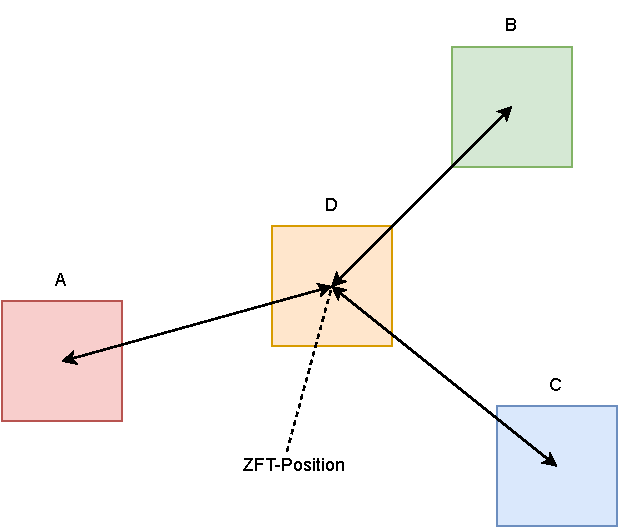
\includegraphics[scale=0.75]{img/zft.pdf}
                \caption{ZFT-Position}
                \label{fig:zft-position}
            \end{figure}
            Zur Bestimmung der ZFT-Position werden die Kräftegleichungen (\ref{equ:Kräftegleichungen})
            null gesetzt und nach der ZFT-Position ($x_i^0$, $y_i^0$) umgestellt sodass
            die Gleichungen (\ref{equ:zft-position}) gebildet werden können \cite{layout}[S. 107].
            \begin{equation}
                \label{equ:Kräftegleichungen}
                \sum_{j} w_{ij} \cdot (x_j^0-x_i^0) = 0~~
                \sum_{j} w_{ij} \cdot (y_j^0-y_i^0) = 0
            \end{equation}
            \begin{equation}
                \label{equ:zft-position}
                x_i^0 = \frac{\sum_{j} w_{ij} \cdot x_j}{\sum_{j} w_{ij}}~~
                y_i^0 = \frac{\sum_{j} w_{ij} \cdot y_j}{\sum_{j} w_{ij}}
            \end{equation}

        \subsection{Grober Ablauf}
            Der grobe Ablauf der Kräfteplatzierung besteht zunächst darin, eine Initialplatzierung zu finden.
            War dies erfolgreich, werden iterativ die ZFT-Position aller Blöcke berechnet.
            Ist die ZFT-Position frei, kann der aktuell betrachtete Block auf die freie Position verschoben werden.
            Ist die Zielposition belegt, muss eine Belegungsoption (\ref{sec:beleungsoptionen}) angewandt werden.
            Ist dies geschehen, wird der nächste Block betrachtet.
            Dies geschieht so lange, bis eine Abbruchbedingung erfüllt ist \cite{layout}[S. 108].

            \begin{enumerate}
                \item Zufällige Initialplatzierung
                \item Berechnen der ZFT-Position des aktuellen Blocks
                        \begin{itemize}
                            \item ZFT-Position ist frei $\rightarrow$ Block auf ZFT-Position verschieben 
                            \item ZFT-Position ist belegt $\rightarrow$ Belegungsoption (\ref{sec:beleungsoptionen}) wählen
                        \end{itemize}
                \item Schritt zwei wiederholen bis Abbruchbedingung erfüllt ist
            \end{enumerate}

        \subsection{Belegungsoptionen}\label{sec:beleungsoptionen}
            \begin{itemize}
                \item Verschieben des Blockes möglichst zu einer Zellenposition nahe der ZFT-Position
                \item Berechnen der Kostenveränderung beim Austausch von zwei Blöcken. Bei verringerten Kosten werden die Blöcke getauscht
                \item \textbf{Chain Move}: Der zu verschiebende Block wird an die Zielposition verschoben,
                    ohne die Kostendifferenz zu berechnen. Der verdränge Block wird auf die nächstgelegende Position verschoben.
                    Ist diese auch belegt, kommt es zu einer Kettenverschiebung (Chain Move)
                \item \textbf{Ripple Move}: Der zu verschiebende Block wird an die Zielposition verschoben und fixiert.
                    Die ZFT-Position des verdrängten Blockes wird berechnet und nach demselben Prinzip verschoben.
                    Dies geschieht so lange, bis alle Blöcke fixiert bzw. platziert sind.
            \end{itemize}\cite{layout}[S. 107f]

            
            





       
        



\chapter{Umsetzung}
    Die Entwicklung der Platzierungssoftware erfolgte in Java-SE 11.
    Der grobe Ablauf des Programmes besteht darin, die Netzliste sowie die fixierten Pads
    einzulesen und daraus ein Graphen zu erstellen.
    Dadurch, dass es im Praktikum nur eine relevante FPGA-Architektur zu betrachten gab,
    wurde vom Einlesen der *.arch Datei abgesehen und die benötigten Parameter wurden über
    Konstanten direkt im Programmcode abgelegt. Wurde der Graph erfolgreich erstellt wird
    eine Initialplatzierung vorgenommen. 
    Kapitel (\ref{sec:init}) beschreibt hierbei die vom Grundalgorithmus abweichende Vorgehensweise
    um die Ergebnisse der Platzierung zu Optimieren. Nach Abschluss der Initialplatzierung
    beginnt die eigentliche Optimierung der Platzierung. Kapitel (\ref{sec:algo}) geht dabei auf die genauen
    Einzelheiten des Algorithmus ein.
    Nach Abschluss des Algorithmus wird aus der aktuellen Platzierung die
    Platzierungsdatei erstellt und ausgegeben.


    \begin{figure}[H]
        \centering
        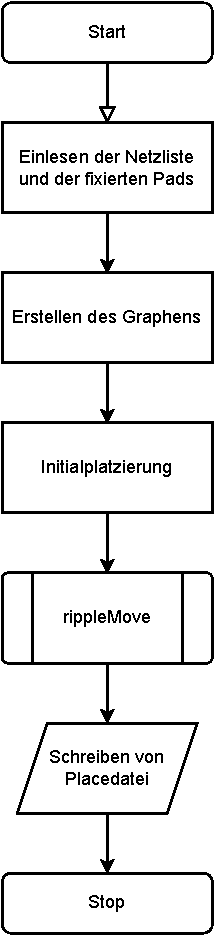
\includegraphics[scale=0.75]{img/Programm-flowchart.pdf}
        \caption{Programmablaufplan}
        \label{fig:program-flowchart}
    \end{figure}

        

    \section{Programmstruktur}

        Abbildung (\ref{fig:uml}) zeigt das UML-Diagramm des Programmes.
        Die Hauptlogik des Programmes befindet sich in der FPGA-Klasse,
        die zuständig für die Platzierung der Logikblöcke ist.
        Als wichtigste Komponente gilt der Graph, der durch die die eingelesenen Blöcke sowie die
        fixierten Pads erstellt wird und der FPGA-Instanz beim Instanziieren übergeben wird.
        Über die Methoden \textit{initPlace} oder \textit{randomPlace} wird eine Initialplatzierung vorgenommen.
        Des weiteren wird über die Methode \textit{rippleMove} die eigentliche Optimierung der Platzierung
        vorgenommen.
        \begin{figure}[H]
            \centering
            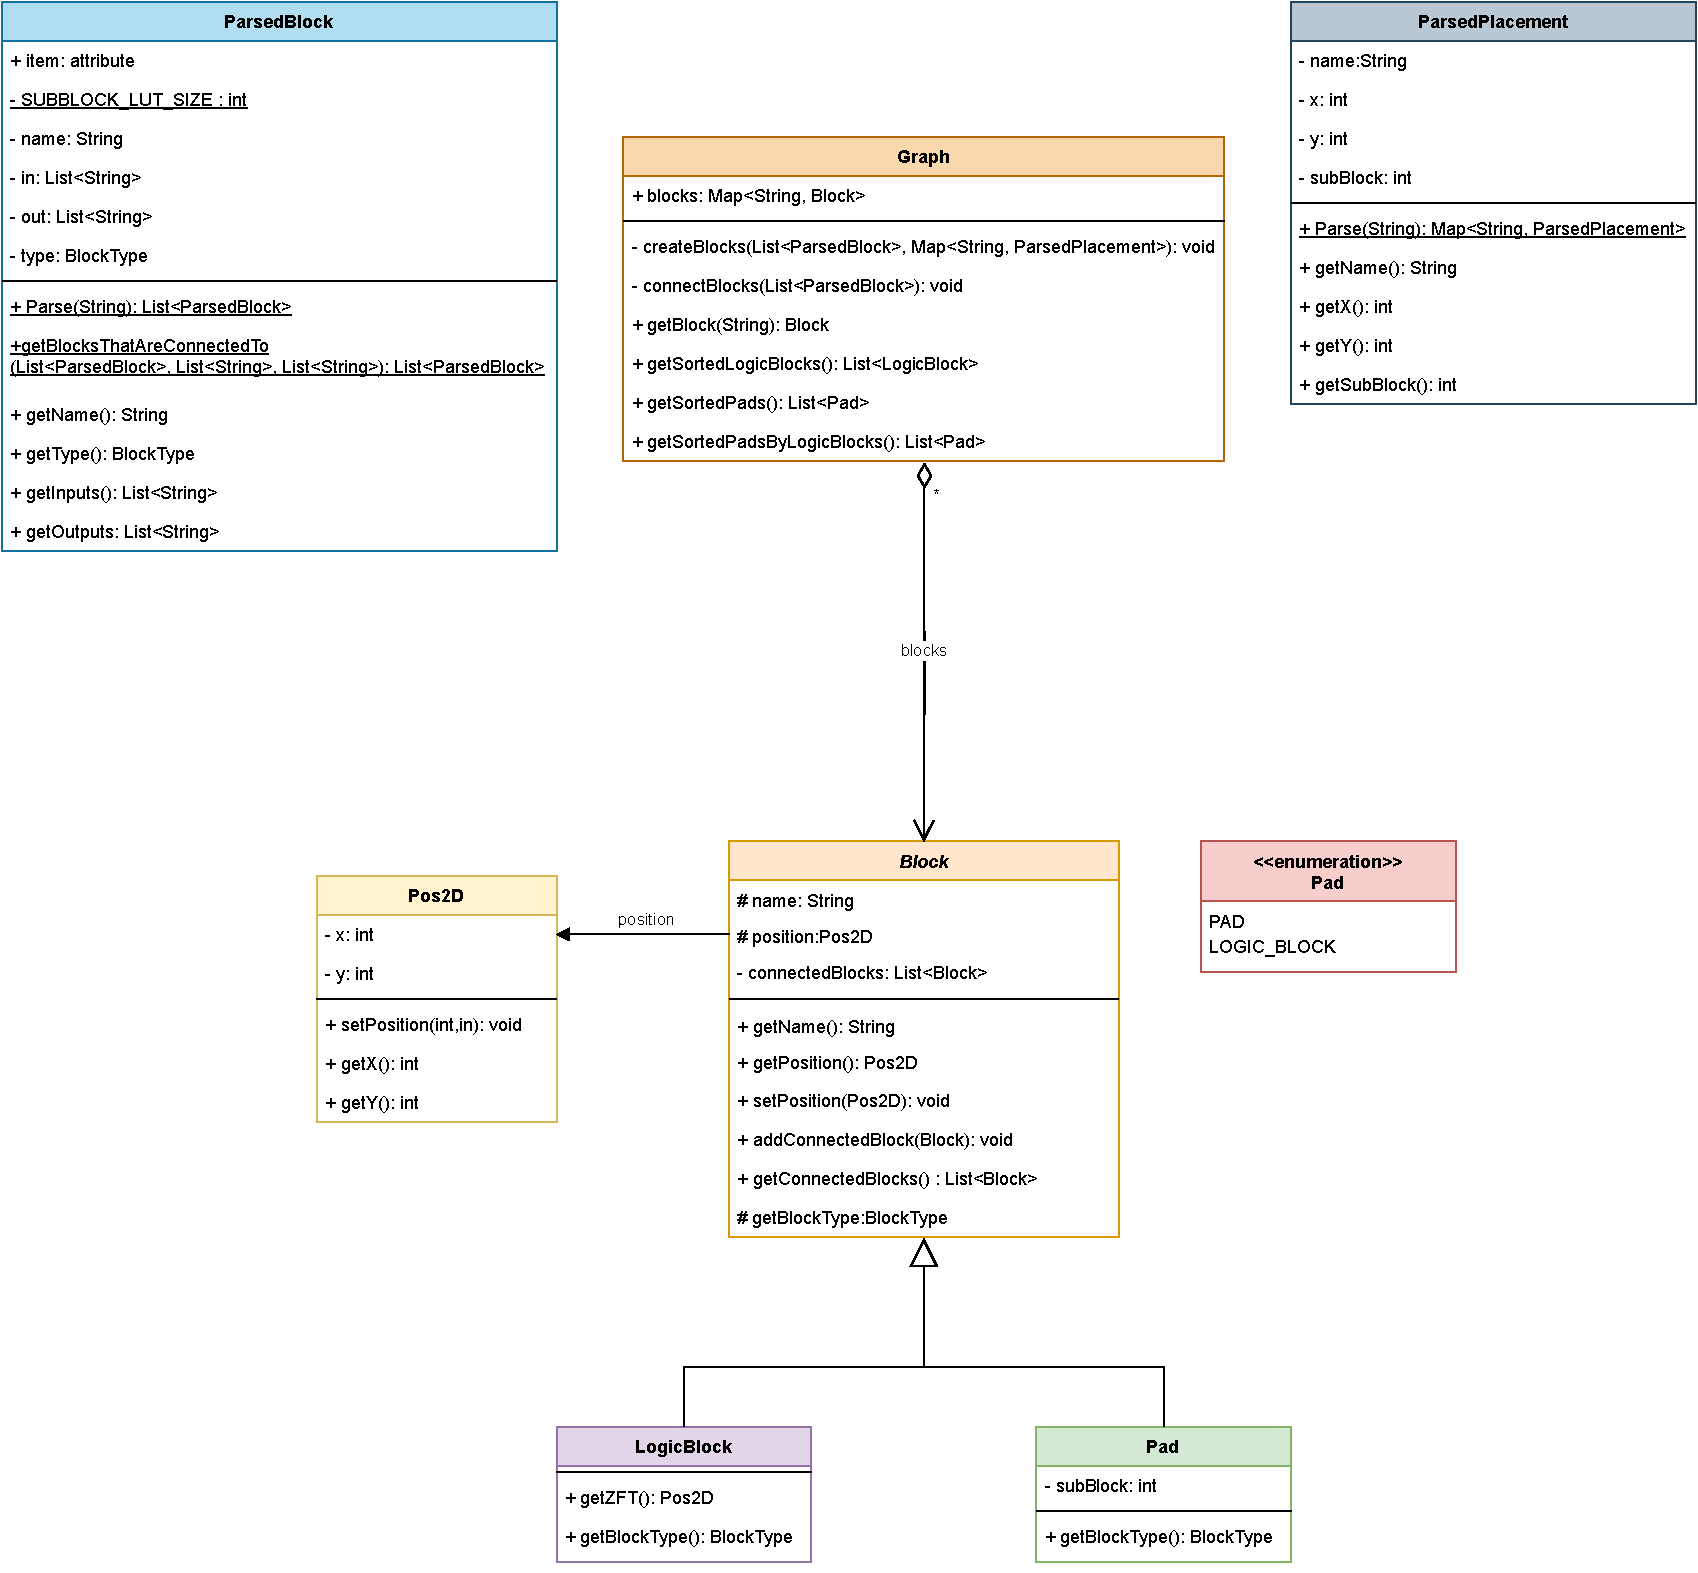
\includegraphics[width=\textwidth]{img/UML.pdf}
            \caption{UML Diagramm}
            \label{fig:uml}
        \end{figure}

    
        
    \section{Initialplatzierung}\label{sec:init}
     

    \section{Algorithmusablaufplan}\label{sec:algo}
        Zunächst werden die Logikblöcke absteigend nach ihrem Verbindungsgrad sortiert.
        Das heißt, dass Blöcke mit mehr Verbindungen weiter vorne in der Liste stehen.
        Dies hat den Vorteil, dass diese Blöcke besser platziert werden können.
        Als Nächstes werden die Blöcke iterativ durchlaufen und für jeden Block die ZFT-Position ermittelt.
        \\
        Ist die Zielposition schon fixiert, das heißt, dass ein anderer Block in
        diesem Iterationsschritt auf die Zielposition gesetzt wurde, wird
        Zunächst der rippleIteration Zähler erhöht und verglichen,
        ob dieser größer bzw. gleich der \textit{maxRippleIteration} Variable ist.
        Ist dies der Fall, wird in der Nähe der Zielposition die nächste freie
        Zelle gesucht und der aktuelle Block auf diese Position gesetzt.
        Des Weiteren wird die maxIteration Zählervariable dekrementiert,
        alle Fixierungen werden gelöst und der Algorithmus beginnt eine neue Iteration. 
        \\
        In dem Fall, dass die \textit{maxRippleIterations} nicht überschritten wurde,
        wird die beste Position in der Nähe der Zielposition gesucht.
        Dabei werden alle anliegenden Positionen betrachtet und die Position ausgewählt,
        an dem der aktuelle Block der niedrigsten Kraft ausgesetzt ist.
        Die neue Zielposition wird daraufhin wieder auf die drei Hauptbedingungen geprüft.
        \\
        Ist die Zielposition nicht fixiert und der Block ist schon auf seiner Zielposition
        werden die \textit{rippleIteration} Variable zurückgesetzt und die Zielposition fixiert.
        \\
        Ist die Zielposition jedoch belegt und nicht fixiert, wird der aktuelle Block
        auf die Zielposition gesetzt, die Position fixiert, der \textit{rippleIteration} Zähler zurückgesetzt
        und der verdrängte Block wird auf den aktuellen Block gesetzt.
        Als Nächstes startet der Algorithmus an der Stelle, an dem die ZFT-Position für den
        aktuellen Block (verdrängter Block) berechnet wird.
        Als letzte Bedingung kann die Zielposition unbelegt sein.
        Ist dies der Fall wird der aktuelle Block auf die Zielposition gesetzt,
        die Position fixiert und der \textit{rippleIteration} Zähler zurück gesetzt.
        Ist der \textit{maxIterations} auf Null dekrementiert worden wird der Algorithmus beendet.

        \begin{figure}[H]
            \centering
            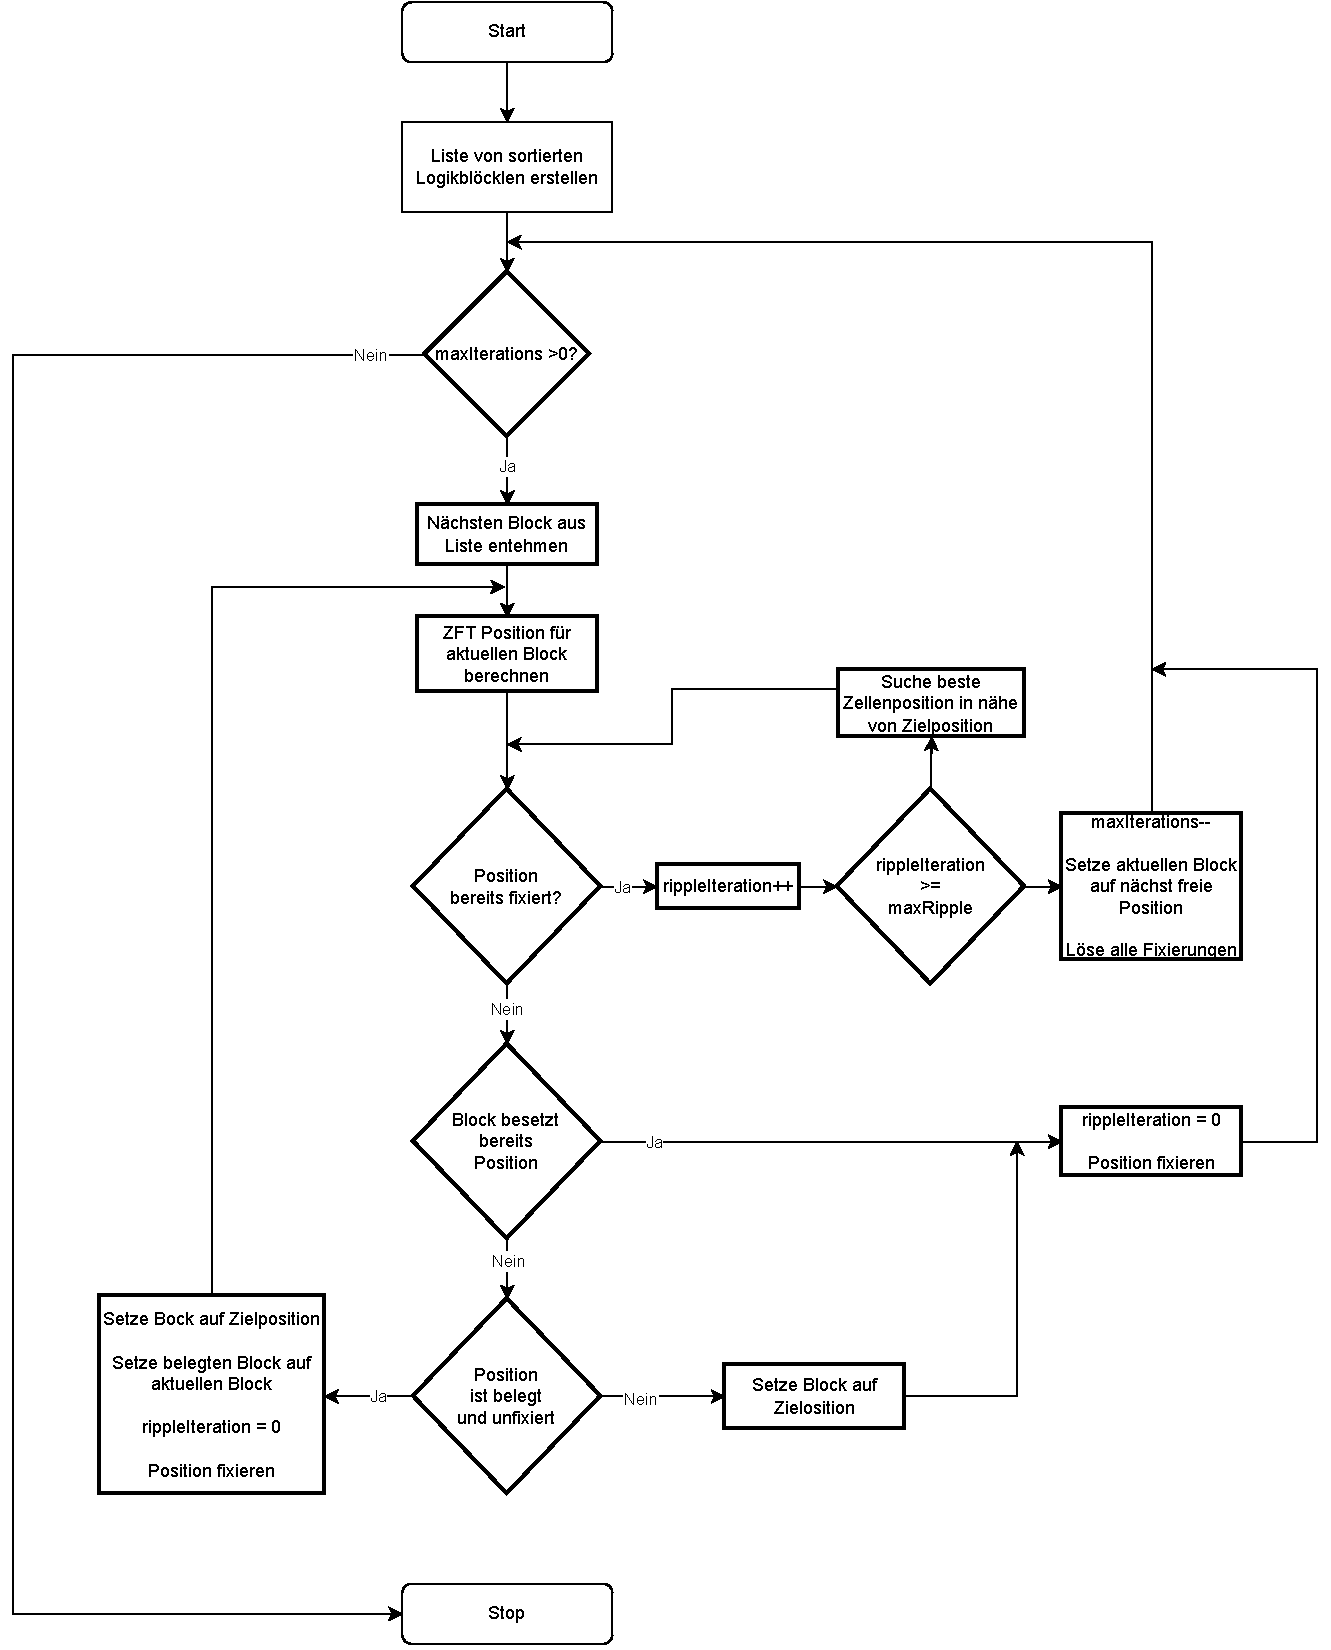
\includegraphics[width=\textwidth]{img/flowchart.pdf}
            \caption{Algorithmusablaufplan}
            \label{fig:algo-flowchart}
        \end{figure}

\chapter{Auswertung}

    Im folgenden Kapitel werden die Ergebnisse ausgewertet und in Relation zu den Benchmarks von VPR gesetzt.
    Zunächst werden in Kapitel (\ref{sec:result-init}) die zwei verschiedenen Initialplatzierungen miteinander
    verglichen. Des Weiteren werden in Kapitel (\ref{sec:result-costs}) die Kosten der Platzierung
    der jeweiligen Benchmarks mit den Platzierungskosten von VPR verglichen.
    Abschließend werden in Kapitel (\ref{sec:result-routing}) die Ergebnisse der vorgenommenen
    Verdrahtung durch VPR verglichen.
    Alle Benchmarks wurden dabei mit einer \textit{maxIterations} von 1000
    und einer \textit{maxRippleIterations} von 20 ausgeführt

    \section{Initialplatzierung}\label{sec:result-init}

        Die Ergebnisse der Platzierung sind unter anderem abhängig von der Initialplatzierung.
        Daher wird die in dieser Arbeit entwickelte Initialplatzierung in diesem Kapitel mit einer
        zufälligen Initialplatzierung verglichen.
        Als Vergleichsgrößen werden die Laufzeit des Gesamtalgorithmus sowie die
        Platzierungskosten verwendet. Dabei gilt für beide Größen,
        dass ein niedrigerer Wert ein besseres Endergebnis darstellt. Tabelle (\ref{tab:init})
        stellt die oben genannten Zusammenhänge tabellarisch dar. Die Differenzspalte ist so zu verstehen,
        dass ein negativer Wert ein besseres Ergebnis darstellt.
        Für die Platzierungen ist die Laufzeit jedoch nicht ausschlaggebend.
        Eine höhere Laufzeit kann in manchen Fällen in Kauf genommen werden, um damit die
        Platzierungskosten niedriger zu halten.
        \\
        Auffällig ist, dass nicht jeder Benchmark von der
        ZFT-Initialplatzierung profitiert. Wie in Kapitel (\ref{sec:init}) erwähnt, ist dies damit zu erklären,
        dass die berechnete ZFT-Position für manche Blöcke nicht exakt berechnet werden kann und somit
        die Initialplatzierung nicht ideal ist. Des Weiteren ist denkbar,
        dass die Zufallsplatzierung durch Zufall eine idealere Initialplatzierung für das iterative
        Verfahren der Kräfteplatzierung findet.
        \\
        In diesem Fall kann durch die ZFT-Initialplatzierung in 11 von 20 Fällen eine bessere
        Platzierung erzielt werden. Zu erwähnen ist auch, dass sich in 8 von 11 Fällen zusätzlich die
        Laufzeit erhöht.

        \begin{center}
            \begin{longtable}{| l | r | r | r | r | r | r |}
                \hline
                \multirow{2}*{\textbf{Benchmark}}  & \multicolumn{2}{|c|}{\textbf{ZFT-Platzierung}} & \multicolumn{2}{|c|}{\textbf{Zufallsplatzierung}} & \multicolumn{2}{|c|}{\textbf{Differenz (\%)}}\\ \cline{2-7}
                                &   Zeit (ms) & Kosten      &   Zeit (ms)   &    Kosten     &   Zeit    &   Kosten  \\ \hline
                    alu4        &   22347   &   390,582     &   22389       &    391.755    & -0.19     & -0.30   \\ \hline
                    apex2       &   35065   &   538,017     &   31763       &    531.647    & 10.40     & 1.20   \\ \hline    
                    apex4       &   13855   &   310,617     &   13833       &    299.461    & 0.16      & 3.73   \\ \hline        
                    bigkey      &   16534   &   505,461     &   15362       &    515.345    & 7.63      & -1.92   \\ \hline        
                    clma        &   408551  &   3555,85     &   507620      &    3493.84    & -19.52    & 1.77   \\ \hline        
                    des         &   2272    &   368,297     &   1858        &    368.784    & 22.28     & -0.13   \\ \hline        
                    diffeq      &   26617   &   385,295     &   25555       &    385.582    & 4.16      & -0.07   \\ \hline        
                    dsip        &   22176   &   456,205     &   20358       &    460.81     & 8.93      & -1.00   \\ \hline        
                    elliptic    &   346639  &   1256,4      &   319950      &    1314.94    & 8.34      & -4.45   \\ \hline         
                    ex5p        &   18487   &   268,953     &   16410       &    276.82     & 12.66     & -2.84   \\ \hline        
                    ex1010      &   123064  &   1266,36     &   108375      &    1239.9     & 13.55     & 2.13   \\ \hline        
                    frisc       &   138902  &   1245,97     &   142276      &    1359.29    & -2.37     & -8.34   \\ \hline        
                    misex3      &   14292   &   340,409     &   10634       &    337.241    & 34.40     & 0.94   \\ \hline        
                    pdc         &   213463  &   1731,39     &   158013      &    1725.91    & 35.09     & 0.32   \\ \hline        
                    s298        &   50932   &   538,604     &   48419       &    538.008    & 5.19      & 0.11   \\ \hline        
                    s38417      &   210034  &   1977,98     &   187441      &    1893.73    & 12.05     & 4.45   \\ \hline        
                    s38584.1    &   1179389 &   2621,59     &   884384      &    2701.24    & 33.36     & -2.95   \\ \hline        
                    seq         &   33346   &   465,327     &   35338       &    464.718    & -5.64     & 0.13   \\ \hline        
                    spla        &   101775  &   1188,14     &   98363       &    1218.62    & 3.47      & -2.50   \\ \hline        
                    tseng       &   8084    &   213,566     &   8445        &    230.618    & -4.27     & -7.39   \\ \hline        
                \caption{Kostenfunktionen und Laufzeit unterschiedlicher Initialplatzierung}
                \label{tab:init}
            \end{longtable}
        \end{center}



    \section{Platzierungskosten}\label{sec:result-costs}

        In diesem Kapitel werden die Ergebnisse der Platzierungen,
        die durch VPR und durch den entwickelten Algorithmus berechnet wurden, miteinander verglichen.
        Je niedriger die Kosten, desto besser ist das Endergebnis. Die Tabelle (\ref{tab:costs})
        stellt die Ergebnissee der 20 Benchmarks dar. Eine negative Differenz bedeutet,
        dass die VPR Platzierung um den jeweiligen prozentualen Wert weniger Platzierungskosten verursacht.
        Die Ergebnisse der Kräfteplatzierung sind bis zu $\approx 75 \%$
        schlechter als die der VPR-Platzierung.\\
        Dabei ist zu erwähnen, dass VPR einen Algorithmus verwendet
        der auf Simulated annealing zurückzuführen ist.
        Dieser ist ein weit verbreiteter Algorithmus und liefert sehr gute Ergebnisse.
        Dies bedeutet im Umkehrschluss, dass die Ergebnisse schwer miteinander zu vergleichen sind. 

        \begin{center}
            \begin{longtable}{| l | r | r | r |}
                \hline
                \textbf{Benchmark}  & \textbf{ZFT-Kosten} & \textbf{VPR-Kosten} & \textbf{Differenz (\%)} \\
                \hline
                    alu4        &   390,582     &   190,135     &   -51,32 \\ \hline
                    apex2       &   538,017     &   269,765     &   -49,86 \\ \hline    
                    apex4       &   310,617     &   179,329     &   -42,27 \\ \hline        
                    bigkey      &   505,461     &   185,977     &   -63,21 \\ \hline        
                    clma        &   3555,85     &   1387,05     &   -60,99 \\ \hline        
                    des         &   368,297     &   227,843     &   -38,14 \\ \hline        
                    diffeq      &   385,295     &   146,394     &   -62,00 \\ \hline        
                    dsip        &   456,205     &   169,991     &   -62,74 \\ \hline        
                    elliptic    &   1256,4      &   457,203     &   -63,61 \\ \hline         
                    ex5p        &   268,953     &   162,012     &   -39,76 \\ \hline        
                    ex1010      &   1266,36     &   655,429     &   -48,24 \\ \hline        
                    frisc       &   1245,97     &   515,59      &   -58,62 \\ \hline        
                    misex3      &   340,409     &   190,205     &   -44,12 \\ \hline        
                    pdc         &   1731,39     &   898,44      &   -48,11 \\ \hline        
                    s298        &   538,604     &   203,949     &   -62,13 \\ \hline        
                    s38417      &   1977,98     &   671,75      &   -66,04 \\ \hline        
                    s38584.1    &   2621,59     &   657,87      &   -74,91 \\ \hline        
                    seq         &   465,327     &   247,658     &   -46,78 \\ \hline        
                    spla        &   1188,14     &   593,969     &   -50,01 \\ \hline        
                    tseng       &   213,566     &   92,0471     &   -56,90 \\ \hline        
                \caption{Kosten der Platzierungen im Vergleich zu VPR}
                \label{tab:costs}
            \end{longtable}
        \end{center}

    \section{Kritischer Pfad und Kanalbreite}\label{sec:result-routing}

        Im folgenden Kapitel werden die Ergebnisse der Verdrahtungen, die durch VPR durchgeführt wurden,
        miteinander verglichen. Dabei hat VPR jeweils die vorgegebenen Platzierungsbenchmarks sowie die
        berechneten Platzierungen durch die entworfene Software verdrahtet.
        Die wichtigsten Kenngrößen nach dem Verdrahtungsschritt sind die Kanalbreite
        sowie die Dauer des kritischen Pfades. Beide Werte sind je besser,
        desto niedriger sie sind und werden in Tabelle (\ref{tab:routing}) dargestellt.
        Die negativen Werte in der Differenzspalte besagen, dass das VPR-Routing eine
        niedrigere Kanalbreite bzw. einen niedrigeren kritischen Pfad verursacht.
        Dass hierbei das VPR-Routing besser ist, liegt daran, dass wie schon in Kapitel (\ref{sec:result-costs})
        erläutert die Platzierungskosten geringer sind. 
        Dementsprechend kann einfacher und mit niedrigerer Kanalbreite
        geroutet werden. Die Differenz der Kanalbreite hat jedoch keinen direkten Zusammenhang mit der
        Differenz des kritischen Pfades, wie das Beispiel des Benchmarks \textit{bigkey} oder \textit{des} zeigt.
        Obwohl in beiden Fällen die Kanalbreite im ZFT-Routing weit aus höher ist als im VPR-Routing, ist
        die Dauer des kritischen Pfades nur $\approx 8\%$ bzw $\approx 6\%$ niedriger.


        \begin{center}
            \begin{longtable}{| l | r | r | r | r | r | r |}
                \hline
                \multirow{2}*{\textbf{Benchmark}}  & \multicolumn{2}{|c|}{\textbf{ZFT-Routing}} & \multicolumn{2}{|c|}{\textbf{VPR-Routing}} & \multicolumn{2}{|c|}{\textbf{Differenz (\%)}}\\ \cline{2-7}
                                &   Kanalbreite &   K. Pfad     &   Kanalbreite &   K. Pfad  &   Kanalbreite &   K. Pfad\\ \hline
                    alu4        &   22  &   1.54E-07    &   11  &   1.12E-07    &   -50.00  &   -27.50   \\ \hline
                    apex2       &   24  &   2.01E-07    &   12  &   1.41E-07    &   -50.00  &   -29.87   \\ \hline    
                    apex4       &   21  &   1.47E-07    &   13  &   1.31E-07    &   -38.10  &   -10.62   \\ \hline        
                    bigkey      &   23  &   1.14E-07    &   6   &   1.06E-07    &   -73.91  &   -7.40    \\ \hline        
                    clma        &   36  &   4.11E-07    &   13  &   2.54E-07    &   -63.89  &   -38.30   \\ \hline        
                    des         &   12  &   1.29E-07    &   8   &   1.21E-07    &   -33.33  &   -5.66    \\ \hline        
                    diffeq      &   21  &   1.84E-07    &   8   &   8.82E-08    &   -61.90  &   -52.11   \\ \hline        
                    dsip        &   23  &   9.21E-08    &   6   &   7.98E-08    &   -73.91  &   -13.44   \\ \hline        
                    elliptic    &   32  &   2.55E-07    &   11  &   1.83E-07    &   -65.63  &   -28.45   \\ \hline         
                    ex5p        &   22  &   1.29E-07    &   14  &   1.09E-07    &   -36.36  &   -15.16   \\ \hline        
                    ex1010      &   22  &   2.87E-07    &   11  &   2.48E-07    &   -50.00  &   -13.61   \\ \hline        
                    frisc       &   27  &   3.01E-07    &   13  &   1.69E-07    &   -51.85  &   -43.85   \\ \hline        
                    misex3      &   20  &   1.34E-07    &   12  &   1.06E-07    &   -40.00  &   -20.86   \\ \hline        
                    pdc         &   34  &   3.17E-07    &   18  &   2.39E-07    &   -47.06  &   -24.52   \\ \hline        
                    s298        &   22  &   2.97E-07    &   8   &   1.98E-07    &   -63.64  &   -33.33   \\ \hline        
                    s38417      &   26  &   2.81E-07    &   8   &   1.77E-07    &   -69.23  &   -36.83   \\ \hline        
                    s38584.1    &   38  &   2.10E-07    &   9   &   1.27E-07    &   -76.32  &   -39.50   \\ \hline        
                    seq         &   23  &   1.39E-07    &   12  &   1.27E-07    &   -47.83  &   -9.00    \\ \hline        
                    spla        &   28  &   2.64E-07    &   14  &   1.76E-07    &   -50.00  &   -33.29   \\ \hline        
                    tseng       &   17  &   1.09E-07    &   7   &   9.00E-08    &   -58.82  &   -17.57   \\ \hline        
                \caption{Kritischer Pfad und Kanalbreite im Vergleich zu VPR}
                \label{tab:routing}
            \end{longtable}
        \end{center}
\chapter{Fazit}


%\pagenumbering{Roman}
%\renewcommand{\thechapter}{\Roman{chapter}}
\newpage
\listoffigures
\listoftables
\printbibliography
\end{document}